\documentclass[11pt]{article}
\usepackage{amsmath}
\usepackage[margin=1in, top=0.5in, bottom=0.5in]{geometry}
\usepackage{libertine}
\usepackage{tikz}
\pagenumbering{gobble}

\title{{\em Modern Climate Change}: a cheat-sheet}
\date{}
\begin{document}
\maketitle

\section{Introduction}
This doc is a collection of notes from the climate science chapters of the
book {\em Modern Climate Change} by Andrew Dessler. It's intended as a quick
reference for the main concepts and formulas for those who've read the book.

\section{Climate history}

\subsection{Recent history}

{\em Temperature anomalies} are the difference between an absolute temperature and a reference
temperature, typically the average temperature over a period of time.

Temperature anomalies can be measured using a network of thermometers that is sparser than
that needed to measure the absolute temperature. The global average temperature
anomaly can be measured using only about 100 thermometer stations. The surface thermometer
record must be adjusted for changes in measurement practices, environmental
changes such as urbanization, and changes in the instruments themselves.

Satellite measurements have been available since 1978. They also need to be adjusted for various
factors including orbital drift and the fact that they measure average atmospheric temperature,
not surface temperature.

The instrumental record shows that the Earth has warmed by about $1.1^\circ$C between the late
1800s and 2010.

Additional indirect evidence of recent climate change includes glacier and ice sheet retreat and
the shrinking of Arctic sea ice.

The top 2000 m of world oceans have warmed by about $0.12^\circ$C between 1960 and 2010.

Ice melt over land and thermal expansion of seawater have caused sea levels to rise by about 100 mm
between 1995 and 2020.

\subsection{Long-term climate record}

Climate data prior to the instrumental record can be obtained from several {\em paleoproxies}, including:

\begin{itemize}
    \item The chemical composition and crystal structure of ice cores.
    \item The chemical composition of air bubbles trapped in ice cores.
    \item Tree rings. (Trees grow more in warm climates.)
    \item Ocean sediments, in particular the prevalance of different species and the chemical
        composition of  fossils.
\end{itemize}

In the last 400M years Earth has alternated between ``icehouse'' and ``greenhouse'' states.
During icehouse phases, ice has extended to $30^\circ$ latitude. During greenhouse phases,
ice disappeared from the poles.

The last greenhouse phase ended about 35M years ago. The peak temperature occurred about 55M years ago,
with the Earth briefly $20^\circ$C warmer than today (Paleocen-Eocene Thermal Maximum).

Until about 3M years ago, temperatures cooled gradually. After that, large ice sheets appeared in the
Northern Hemisphere and oscilations between warm and cold periods appear in the record.

Between approximately 2.5M and 1M years ago, ice ages occured every 41K years. About 1M years ago,
the frequency changed to every 100K years and the amplitude of the temperature changes increased.

In the last 400K years, ice ages have lasted about 100K years and interglacials about 10-30K years.
Cooling took a long time (tens of thousands of years) but warming was rapid (about 10K years).

Atmospheric CO$_2$ concentration in ice cores tracks temperature changes closely.

\section{Radiation and energy balance}

A black body is an (idealized) object that absorbs all radiation that hits it.
It also emits radiation at a rate that depends on its temperature.

The relationship between the temperature of a black body and the peak of its emission spectrum is
given by Wien's law:
\[
\lambda_{\text{max}} = \frac{b}{T}
\]
where $\lambda_{\text{max}}$ is the wavelength of the peak emission ($\mu$m), $b$ is Wien's constant (2897 $\mu$m$\cdot$K),
and $T$ is the temperature (K). Since wavelength and frequency are inversely related, the frequency of the peak emission
increases with temperature. Visible light has wavelengths between 0.4 and 0.8 $\mu$m.
Some examples:
\begin{itemize}
    \item A 1600 K object emits most of its radiation as infrared light but some of its radiation is in the red end of the visible spectrum,
        so it glows ``red hot''.
    \item An incandescent filament has a temperature of 3000K and emits most of its radiation in the infrared spectrum but more of it is in the visible spectrum.
    \item The Sun has a temperature of 6800 K and most of its radiation is in the visible spectrum.
\end{itemize}

The Stefan-Boltzmann law describes the relationship between the temperature of a black body
and the rate at which it emits radiation:
\[
P/a = \sigma T^4
\]
where $P$ is the rate of radiation emission (W), a is the surface area (m$^2$), $T$ is the temperature of the black body (K),
and $\sigma$ is the Stefan-Boltzmann constant, $5.67 \times 10^{-8}$ W/m$^2$K$^4$.

The net change in internal energy of an object is given by the difference between the energy it absorbs and the energy it emits:
\[
\Delta U = E_{\text{in}} - E_{\text{out}}
\]
where $E_{\text{in}}$ is the energy absorbed and $E_{\text{out}}$ is the energy emitted.



\section{Simple climate models}
\[
T = \sqrt[4]{\frac{(n+1)S(1-\alpha)}{4 \sigma}}
\]


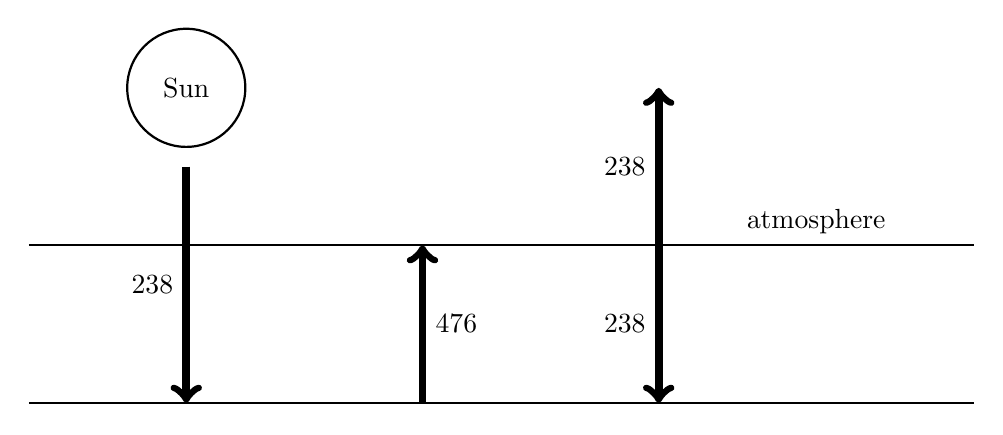
\begin{tikzpicture}[xscale=2]
    % Sun
    \node at (1,4) [circle, draw, thick, minimum size=1.5cm] {Sun};

    % Atmosphere layer
    \draw[thick] (0, 2) -- (6, 2);
    \node at (5, 2.3) {atmosphere};

    % Ground layer
    \draw[thick] (0, 0) -- (6, 0);

    % Arrows
    % sun to earth
    \draw[line width=1mm, ->] (1, 3) -- (1, 0) node[midway, left] {238};
    % earth to atmosphere
    \draw[line width=1mm, ->] (2.5, 0) -- (2.5, 2) node[midway, right] {476};

    % atmosphere to earth
    \draw[line width=1mm, ->] (4, 2) -- (4, 0) node[midway, left] {238};
    % atmosphere to space   
    \draw[line width=1mm, ->] (4, 2) -- (4, 4) node[midway, left] {238};

\end{tikzpicture}

\section{The carbon cycle}
\section{Forcings, feedbacks, and climate sensitivity}

\end{document}
